\chapter{Introduction}

\section[Introduction]{\textbf{Overview}}
As multipliers play a critical role in any digital design. It is necessary to implement faster multipliers occupying lesser area and consuming less power. Multiplication operation can be done using Array multiplier, redundant binary structures, and tree structures but they have problem of larger delay. Vedic mathematics is the name given to the ancient Indian system of mathematics that was rediscovered in early 20th century. Vedic multiplication uses Urdhva Triyakbhyam (Vertically and Cross wise) Sutras. 
%\begin{figure}[htb]
%\centering
%	
\includegraphics[scale=1]{Figures/universe}	
%	\caption{Sample picture of universe }
%	\label{fig:universe}
%\end{figure}


\section[Motivation]{\textbf{Motivation}}

\begin{itemize}
	\item Vedic mathematics helps in simplifying calculations.
	\item High-speed Area Efficient 3 operands Adder provides better speed and less area than carry save adder.\\
\end{itemize}

\section[Problem statement]{\textbf{Problem statement}}

To achieve better speed and area efficient 16x16 Vedic multiplier using High-speed Area Efficient three operands Adder and compare the same using 16x16 Vedic multiplier using Carry Save Adder.
\\
\\
\section[Objectives]{\textbf{Objectives}}
The objectives of the project are
\begin{enumerate}
\item To design a Verilog code and implement 16x16 Vedic multiplier using Carry Save Adder.
\item To design a Verilog code and implement 16x16 Vedic multiplier using High Speed Area Efficient 3 operands Adder.
\item Comparing delay and power consumption for both the adders.
\end{enumerate}

\section[Literature Review]{\textbf{Literature Review}}

To achieve optimal system performance while maintaining physical security, it is necessary to implement the cryptography algorithms on hardware [1] – [3]. Modular arithmetic such as modular exponentiation, modular multiplication and modular addition is frequently used for the arithmetic operations in various cryptography algorithms [4]. Therefore, the performance of the cryptography algorithm depends on the efficient implementation of the congruential modular arithmetic operation. The most efficient approach to implement the modular multiplication and exponentiation is the Montgomery algorithm [5] – [7] whose critical operation is based on three-operand binary addition [6] – [8]. The three-operand binary addition is also a primary arithmetic operation in the linear congruential generator (LCG) based pseudo-random bit generators (PRBG) such as coupled LCG (CLCG) [9], modified dual-CLCG (MDCLCG) [10] and coupled variable input LCG (CVLCG) [11]. Modified dual-CLCG (MDCLCG) is the most secure and highly random PRBG method among all the LCG-based and other existing PRBG methods. It is polynomial-time unpredictable and secure if n \_ 32-bits. Therefore, the security of the MDCLCG enhances with the increase of operand size. However, the area and critical path delay increases linearly since its hardware architecture consists of four three-operand modulo-2n adders, two comparators, four multiplexers area [10]. Hence, the performance of the MDCLCG can be improved by the efficient implementation of the three-operand adder. The three-operand binary addition can be carried out either by using two two-operand adders or one three-operand adder. Carry-save adder (CS3A) is the area-efficient and widely adopted technique to perform the three-operand binary addition in the modular arithmetic used in cryptography algorithms [5] – [8], [12] – [14] and PRBG methods [9] – [11]. However, the longer carry propagation delay in the ripple-carry stage of CS3A seriously influences the performance of the MDCLCG and other cryptography architectures on IoT based hardware devices. To shorten the critical path delay, a parallel prefixed two-operand adder such as Han-Carlson (HCA) can also be used for three-operand binary addition. It reduces the critical path delay in the order of O(log2 n) but increases the area in the order of O(n log2 n) [15]. Therefore, it is necessary to develop an efficient VLSI architecture to carry out the fast three-operand binary addition with minimum hardware resources. Hence, a new high-speed area-efficient adder technique is proposed using pre-compute bitwise addition followed by carry-prefix computation logic to perform the three-operand addition in this paper that consumes considerably less gate area while minimizing the propagation delay in comparison to the HCA-based three-operand adder (HC3A). 



\section[Brief Methodology of the project]{\textbf{Brief Methodology of the project}}
A 2x2 Vedic Multiplier is used to design 16x16 Vedic multiplier using carry save adder and high-speed area efficient (HSAE) adder. The fig.~\ref{fig:x1} shows the design of 2x2 Vedic Multiplier as shown below.
\begin{figure}[htb]
\centering
	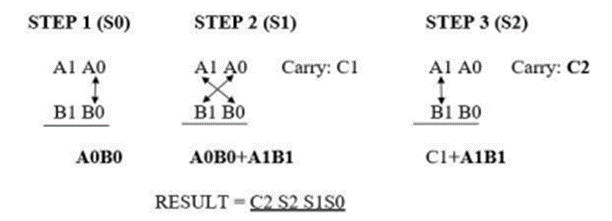
\includegraphics[scale=1]{Figures/x1}	
	\caption{2x2 Vedic Multiplier}
	\label{fig:x1}
\end{figure}
The design of 4x4 Vedic Multiplier using 2x2 Vedic Multiplier and CSA is shown below in fig.~\ref{fig:x2}
\begin{figure}[htb]
	\centering
	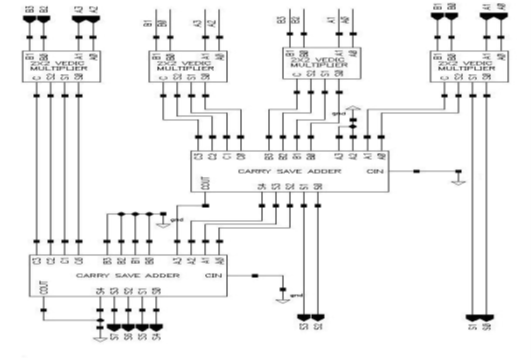
\includegraphics[scale=1]{Figures/x2}	
	\caption{4x4 Vedic Multiplier}
	\label{fig:x2}
\end{figure}
Similar to 4x4 Vedic Multiplier, the 8x8 and 16x16 Vedic Multipliers are designed using CSA and HSAE adder.
$S'\_{i}= a\_{i} \oplus b\_{i} \oplus c\_{i}$

\section[Organization of the report]{\textbf{Organization of the report}}

This report is organized as follows. Write the discussions in each chapter. A sample is as follows.
\begin{itemize}
\item Chapter 2 discusses the fundamentals of three-operand binary adder techniques.
\item Chapter 3 discusses the design of 16 x 16 Vedic multiplier.
\item Chapter 4 discusses the results and discussions.
\item Chapter 5 discusses the conclusion and future scope.
\end{itemize}

.